\section{Introduction}

Aerosols play an important role in regulating climate change. In the context of global climate change, this regulation is global. To understand the impact of aerosols on global climate change, global aerosol observations are urgently needed.

At present, the observation data of aerosols are still scattered in a large number of documents and other types of storage media. For readers who need data, it is a cumbersome and unpleasant process to move between data platforms. Moreover, the traditional literature review is fixed in the form of papers. For the author, it is necessary to read a large amount of literature for statistical compilation, and every few years need to be updated to ensure the real-time statistical knowledge of such documents. The workload is large and cumbersome. For the reader, in order to quickly acquire such statistical knowledge, it is necessary to search for the review literature and judge their authority. The acquired knowledge is also limited by the region, year, etc. that the author wants to display.

In the face of a large number of intricate data, relying on traditional literature collection methods, it is difficult to extract aerosol data in massive documents quickly and efficiently, and the practice of reviewing for many years is far from satisfying the data iteration. In this article, we will present a solution to the problem by building an aerosol knowledge base. And on the basis of the establishment of the knowledge base, we have built the world's first comprehensive literature knowledge online website system dedicated to the aerosol field, giving full play to the role of literature data.

This article is divided into six parts to introduce this website system, the first section: related work; the second section: knowledge base design; the third section: knowledge service design; the fourth section: user experience: the fifth section: data expansion; Section: Conclusion.

\section{Related Wprk}
Our work intends to leverage the knowledge and services of the literature data, and we have built the world's first comprehensive online knowledge website system for the aerosol field. These technologies have attracted many efforts from different research fields. In this section, we will review the work in each area, as our work is inspired by the literature and draws lessons from previous methods.


\subsection{Knowledge Base}

Since 2002, R.Crow first proposed the concept of Institutional Repository (IR) to actively build institutional knowledge bases in universities and institutions libraries at home and abroad. It has been nearly 16 years, but the development of knowledge base is still trying. And groping, there is no ready-made road map. This is also a big problem that the system needs to solve in the design.

At present, the commonly used knowledge bases in China include Zhiwang, Wanfang, Baidu Academic, and the knowledge bases of major universities. There are Web of science and Nature in the world. However, most of them only provide the functions of paper search and keyword indexing. Some domestic websites can provide services for checking papers. However, such data search methods are too broad, and they cannot quickly acquire a certain field in a certain period of time. Data trends within and statistical analysis results. This is exactly what we are trying to solve.

\subsection{Knowledge Service Model}
The current society is a service-based society, and the product production economy is gradually transformed into a service economy. The traditional innovation model based on technology is shifting from a user vision. We should also shift our product-centricity to users’ center.

\subsection{Crowdsourcing}
The crowdsourcing method can recruit mass participants through the Internet to complete the work that the machine is difficult to accomplish. Since Howe proposed the concept of crowdsourcing in 2006, the research and application of crowdsourcing has developed rapidly. Due to the diverse backgrounds, low labor costs, and fast task completion, crowdsourcing has developed rapidly and is widely used in image classification, manufacturing, film and television, human-computer interaction, and medicine.

In this article, we will also apply the crowdsourcing method, invite experts and scholars to fill out and submit the data of published articles, so as to expand the database.

\section{IR DESIGN}
The construction of IR requires good management, requires continuous planning, prioritization and coordination of different stakeholders, including academic and academic researchers, libraries, institutional managers, publishers, and even students participating in research (doctors, masters) benefits.

The existence of IR must meet the needs of all parties involved. For this system, we plan, prioritize and coordinate different stakeholders, including experts in academic fields, teaching and research personnel in institutions, students participating in research (doctors, masters), and the interests of the masses, and analyze the interests. The difference between the reality and the needs of the party. See Table 1 for details.

The current literature data of this aerosol knowledge base covers 75 core aerosol-related journals, with more than 13,000 aerosol-related literature data and more than 100,000 abstract data. The paper data covers China, South Korea, Japan, India, Africa, the United States and other countries and continents, as shown in Figure 1.

\begin{figure}
	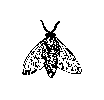
\includegraphics{fly}
	\caption{Paper distribution in world map.}
\end{figure}

In China, the data covers Beijing, Chongqing, Xinjiang, Jiangsu Province, Anhui Province, Taiwan Province, Guangdong Province, Hubei Province, Guizhou Province, Gansu Province, and Shaanxi Province, as shown in Figure 2.

\begin{figure}
	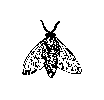
\includegraphics{fly}
	\caption{Paper distribution in chinese map.}
\end{figure}


\section{KNOWLEDGE SERVICE}
We regard knowledge service as a system problem. Starting from the user's needs mining, through the form of questionnaires and interviews, we collect and determine the requirements, systematically apply the theory and method of design to create and plan services: system for regions, wavelengths , the year and other conditions for statistical analysis of the data in the database, and visual display, hope that users can quickly and intuitively obtain statistical knowledge of aerosol data. Services form a process and have value to end users, resulting in high quality services that enhance the user experience.

Different services have different meanings at different times, so service products are often personalized. In this regard, this paper designs adaptive service functions for the knowledge service system based on the exclusive characteristics of the aerosol literature. Therefore, after we get Table 3, we made relevant user surveys for the personnel objects in Table 3 and their interests, in order to determine the service function points.

\subsection{User Questionnaire}
We set up an online questionnaire to collect public information. A total of 20 questionnaires (currently) were collected, including 3 in the aerosol professional field and 17 in the non-aerosol professional field (both students). The questionnaire was in the form of a question. ,including but not limited to:

(1) What is the method for determining the direction of the paper before the paper is written?

(2) In what form do you want to get data in the paper?

(3) In what form do you want to judge your paper after the paper is written?

For this survey, we got a lot of important responses and suggestions. In the process of sorting out the answers, we made clear the determination of the system function. The tentative function points are as follows in Table 2:

\begin{table}
	\caption{Tentative Function Points Questionnaire}
	\label{tab:freq}
	\begin{tabular}{ccl}
		\toprule
		Functions&Proportion\\
		\midrule
		Keyword Query & xx\%\\
		Topic Classification & xx\%\\
		Paper Review & xx\%\\
		Paper Evaluation & xx\%\\
		Paper Template & xx\%\\
		\bottomrule
	\end{tabular}
\end{table}

\subsection{User Interview}
In order to further deepen the user's needs and determine the system functions, we adopted the focus group interview method. We interviewed 100 volunteers, including 50 in the aerosol field (professionals include teachers and students) and 50 non-aerosol professionals (occupations include teachers, students, and other corporate workers). 

Face-to-face user interviews were conducted with a group of 10 people (the same professional). We will first set up different aerosol literature knowledge related project questions based on volunteer career information, record the problem solving needs through the discussion between volunteers, and let the volunteers click on the importance of the functions we selected before. The scale is shown in Figure 3:

\begin{figure*}
	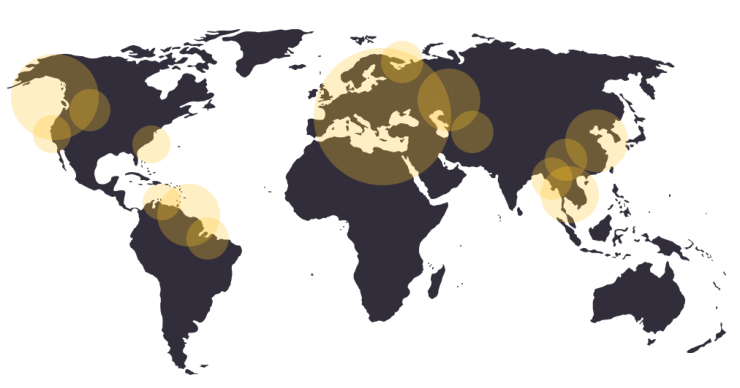
\includegraphics[width=0.8\textwidth]{pic1.pdf}
	\caption{Subscale.}
\end{figure*}

Based on the interview results and the scoring statistics, we removed the “paper template” function points obtained through the questionnaire, and added the “data visualization” function points obtained through focus group interviews. The final score and the determined function points are shown in Table 3:

\begin{table}
	\caption{Final Function Point and Scoring Result}
	\label{tab:freq}
	\begin{tabular}{ccl}
		\toprule
		Functions&Score Result\\
		\midrule
		Keyword Query & xx\\
		Topic Classification & xx\\
		Paper Review & xx\\
		Paper Evaluation & xx\\
		\midrule
		New\\
		Data Visualization & xx\\
		\bottomrule
	\end{tabular}
\end{table}


\subsection{Tables}
Because tables cannot be split across pages, the best
placement for them is typically the top of the page
nearest their initial cite.  To
ensure this proper ``floating'' placement of tables, use the
environment \textbf{table} to enclose the table's contents and
the table caption.  The contents of the table itself must go
in the \textbf{tabular} environment, to
be aligned properly in rows and columns, with the desired
horizontal and vertical rules.  Again, detailed instructions
on \textbf{tabular} material
are found in the \textit{\LaTeX\ User's Guide}.

Immediately following this sentence is the point at which
Table~\ref{tab:freq} is included in the input file; compare the
placement of the table here with the table in the printed
output of this document.

\begin{table}
	\caption{Frequency of Special Characters}
	\label{tab:freq}
	\begin{tabular}{ccl}
		\toprule
		Non-English or Math&Frequency&Comments\\
		\midrule
		\O & 1 in 1,000& For Swedish names\\
		$\pi$ & 1 in 5& Common in math\\
		\$ & 4 in 5 & Used in business\\
		$\Psi^2_1$ & 1 in 40,000& Unexplained usage\\
		\bottomrule
	\end{tabular}
\end{table}

To set a wider table, which takes up the whole width of the page's
live area, use the environment \textbf{table*} to enclose the table's
contents and the table caption.  As with a single-column table, this
wide table will ``float'' to a location deemed more desirable.
Immediately following this sentence is the point at which
Table~\ref{tab:commands} is included in the input file; again, it is
instructive to compare the placement of the table here with the table
in the printed output of this document.


\begin{table*}
	\caption{Some Typical Commands}
	\label{tab:commands}
	\begin{tabular}{ccl}
		\toprule
		Command &A Number & Comments\\
		\midrule
		\texttt{{\char'134}author} & 100& Author \\
		\texttt{{\char'134}table}& 300 & For tables\\
		\texttt{{\char'134}table*}& 400& For wider tables\\
		\bottomrule
	\end{tabular}
\end{table*}
% end the environment with {table*}, NOTE not {table}!

It is strongly recommended to use the package booktabs~\cite{Fear05}
and follow its main principles of typography with respect to tables:
\begin{enumerate}
	\item Never, ever use vertical rules.
	\item Never use double rules.
\end{enumerate}
It is also a good idea not to overuse horizontal rules.


\subsection{Figures}

Like tables, figures cannot be split across pages; the best placement
for them is typically the top or the bottom of the page nearest their
initial cite.  To ensure this proper ``floating'' placement of
figures, use the environment \textbf{figure} to enclose the figure and
its caption.

This sample document contains examples of \texttt{.eps} files to be
displayable with \LaTeX.  If you work with pdf\LaTeX, use files in the
\texttt{.pdf} format.  Note that most modern \TeX\ systems will convert
\texttt{.eps} to \texttt{.pdf} for you on the fly.  More details on
each of these are found in the \textit{Author's Guide}.

\begin{figure}
	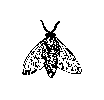
\includegraphics{fly}
	\caption{A sample black and white graphic.}
\end{figure}

\begin{figure}
	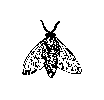
\includegraphics[height=1in, width=1in]{fly}
	\caption{A sample black and white graphic
		that has been resized with the \texttt{includegraphics} command.}
\end{figure}


As was the case with tables, you may want a figure that spans two
columns.  To do this, and still to ensure proper ``floating''
placement of tables, use the environment \textbf{figure*} to enclose
the figure and its caption.  And don't forget to end the environment
with \textbf{figure*}, not \textbf{figure}!

\begin{figure*}
	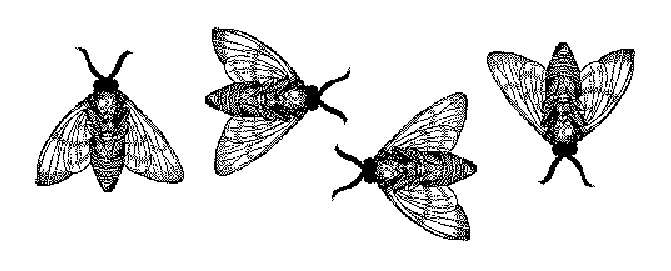
\includegraphics{flies}
	\caption{A sample black and white graphic
		that needs to span two columns of text.}
\end{figure*}


\begin{figure}
	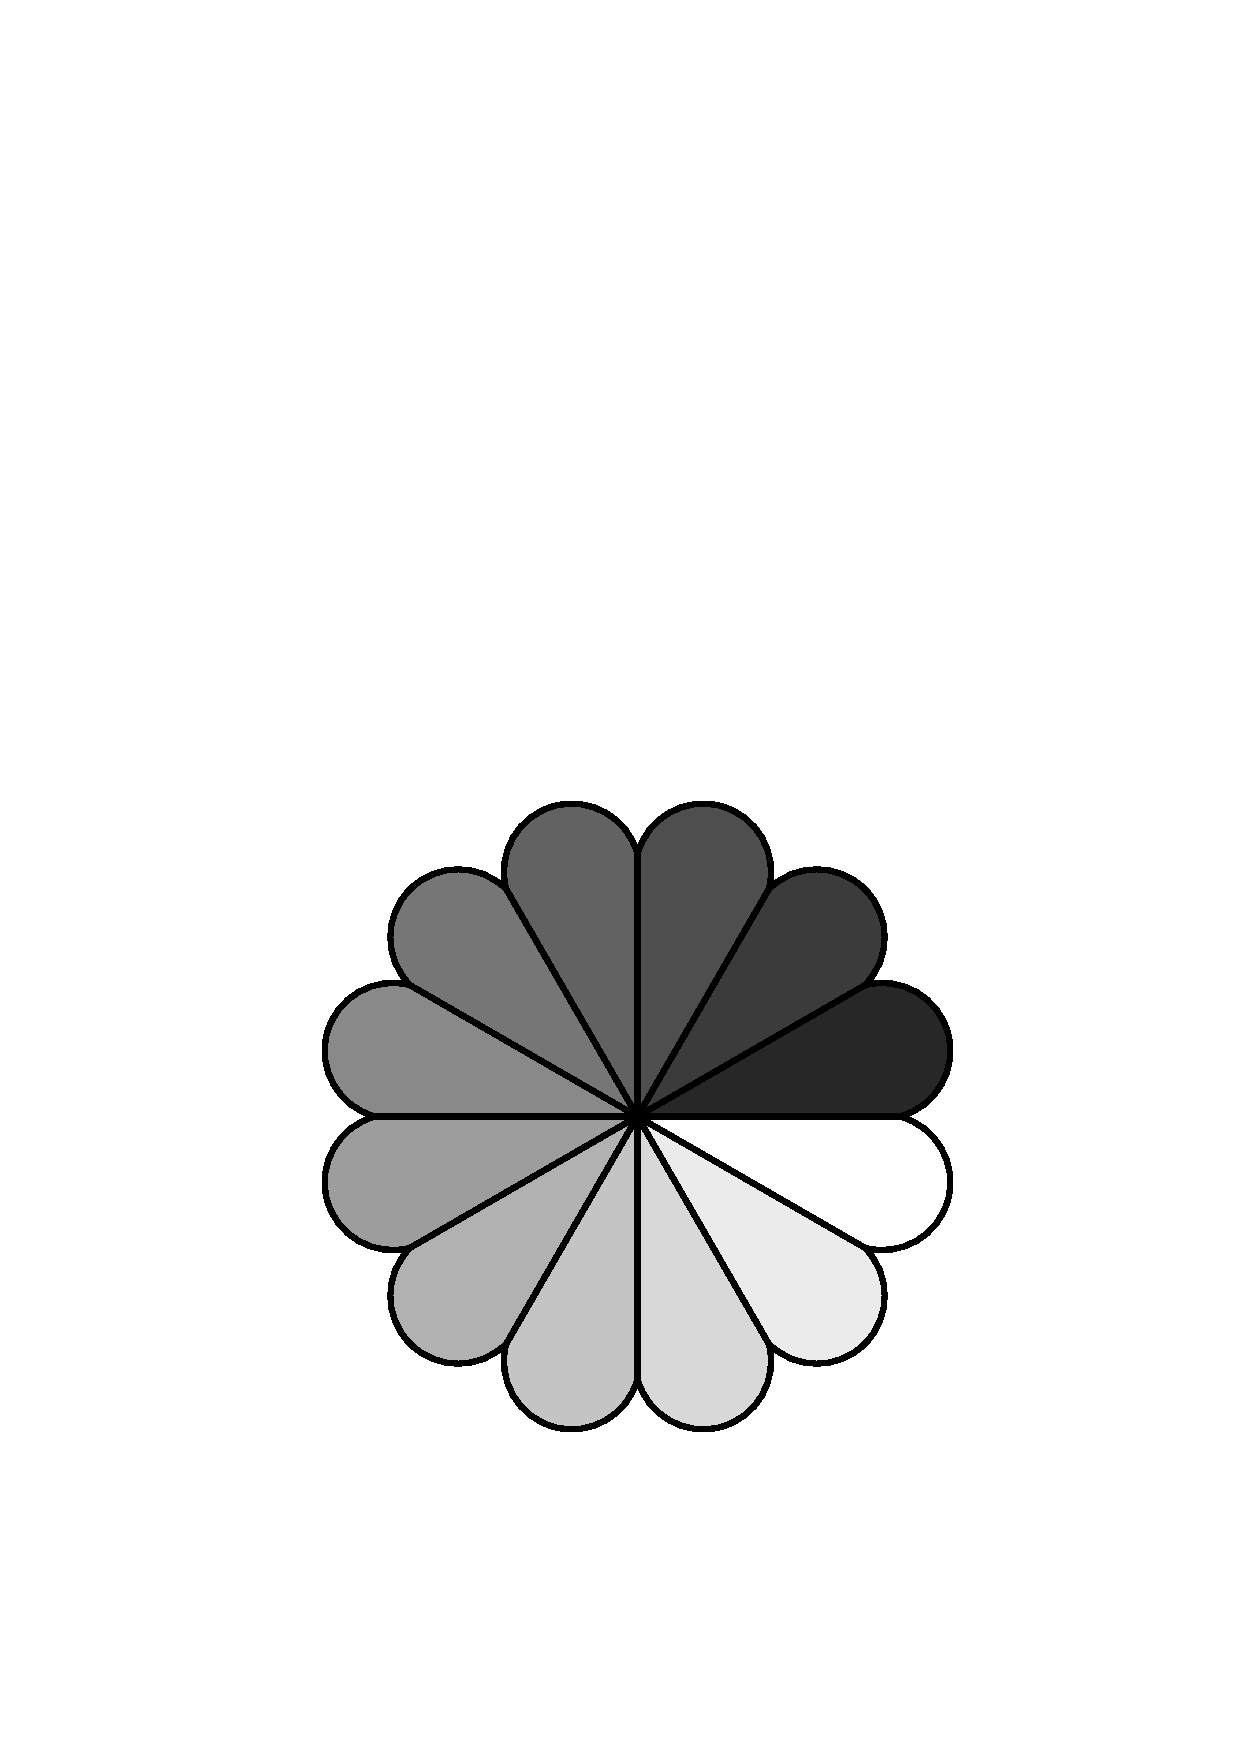
\includegraphics[height=1in, width=1in]{rosette}
	\caption{A sample black and white graphic that has
		been resized with the \texttt{includegraphics} command.}
\end{figure}

\subsection{Theorem-like Constructs}

Other common constructs that may occur in your article are the forms
for logical constructs like theorems, axioms, corollaries and proofs.
ACM uses two types of these constructs:  theorem-like and
definition-like.

Here is a theorem:
\begin{theorem}
	Let $f$ be continuous on $[a,b]$.  If $G$ is
	an antiderivative for $f$ on $[a,b]$, then
	\begin{displaymath}
	\int^b_af(t)\,dt = G(b) - G(a).
	\end{displaymath}
\end{theorem}

Here is a definition:
\begin{definition}
	If $z$ is irrational, then by $e^z$ we mean the
	unique number that has
	logarithm $z$:
	\begin{displaymath}
	\log e^z = z.
	\end{displaymath}
\end{definition}

The pre-defined theorem-like constructs are \textbf{theorem},
\textbf{conjecture}, \textbf{proposition}, \textbf{lemma} and
\textbf{corollary}.  The pre-defined de\-fi\-ni\-ti\-on-like constructs are
\textbf{example} and \textbf{definition}.  You can add your own
constructs using the \textsl{amsthm} interface~\cite{Amsthm15}.  The
styles used in the \verb|\theoremstyle| command are \textbf{acmplain}
and \textbf{acmdefinition}.

Another construct is \textbf{proof}, for example,

\begin{proof}
	Suppose on the contrary there exists a real number $L$ such that
	\begin{displaymath}
	\lim_{x\rightarrow\infty} \frac{f(x)}{g(x)} = L.
	\end{displaymath}
	Then
	\begin{displaymath}
	l=\lim_{x\rightarrow c} f(x)
	= \lim_{x\rightarrow c}
	\left[ g{x} \cdot \frac{f(x)}{g(x)} \right ]
	= \lim_{x\rightarrow c} g(x) \cdot \lim_{x\rightarrow c}
	\frac{f(x)}{g(x)} = 0\cdot L = 0,
	\end{displaymath}
	which contradicts our assumption that $l\neq 0$.
\end{proof}

\section{Conclusions}
This paragraph will end the body of this sample document.
Remember that you might still have Acknowledgments or
Appendices; brief samples of these
follow.  There is still the Bibliography to deal with; and
we will make a disclaimer about that here: with the exception
of the reference to the \LaTeX\ book, the citations in
this paper are to articles which have nothing to
do with the present subject and are used as
examples only.
%\end{document}  % This is where a 'short' article might terminate


\begin{acks}
	The authors would like to thank Dr. Yuhua Li for providing the
	MATLAB code of the \textit{BEPS} method.
	
	The authors would also like to thank the anonymous referees for
	their valuable comments and helpful suggestions. The work is
	supported by the \grantsponsor{GS501100001809}{National Natural
		Science Foundation of
		China}{http://dx.doi.org/10.13039/501100001809} under Grant
	No.:~\grantnum{GS501100001809}{61273304}
	and~\grantnum[http://www.nnsf.cn/youngscientists]{GS501100001809}{Young
		Scientists' Support Program}.
	
\end{acks}
